% !TeX root = ../main.tex

\chapter{數學排版}
\label{ch:math}\index{數學排版}

好啦!這章是 \LaTeX{} 的拿手把戲了。就讓我們就來見識一下 \LaTeX{} 的威力吧!光這一章的內容就可以寫一本厚厚的書了,所以,只能點到為止,先小酌一番。這一章的內容,他們排版精確性,以 PDF 格式的內容為準,HTML 格式的內容,僅供參考。

對於較複雜的數學式子,除非是自行定義巨集,否則 \LaTeX{} 內建所提供的排版數學式子的能力可能會有不足,這時可以使用美國數學協會所開發的 \AmS{}-\LaTeX{}\index{AmS-LaTeX@\AmS{}-\LaTeX{}} 巨集套件,目前所有的 \TeX{} 發行版本應該都會附上,而且也會附上另一套 {\sffamily AMSFonts} 巨集套件及其字型。這個套件的使用,這裡並不做詳細的說明,只在必要的時候附帶提及,可以另外參考系統上所附的 {\ttfamily amsldoc.dvi} 文件及 \textit{The \LaTeX{} Companion} 這本書第八章,這個部份網路上可以抓得到,檔名是 {\ttfamily ch8.pdf},CTAN 有收錄:

\begin{quote}
  \url{http://www.ctan.org/tex-archive/info/companion-rev/ch8.pdf}
\end{quote}

\section{進入數學模式(math mode)的方法}\index{數學模式(math mode)}

我們平常寫文章的模式無法正確處理數學式子間的空間位置,而且要鍵入次方、方根、積分 \chdots{} 等等符號,會有困難,因此,所有的數學式子都得進入數學模式來處理。在數學模式下,不僅大部份文字、符號會採用斜體字,而且空間會另做安排,額外的空白會被 \LaTeX{} 忽略,在數學模式中要鍵入一般的正常文字,要退出數學模式,或者由 \verb|\mbox{}| 或 \verb|\textmr{}| 包圍起來才行。

\LaTeX{} 的數學模式有兩種,一種是和內文排列在一起的隨文數式(math inline mode),他是和一般正常文字混在一起排版的;另外一種是獨立的展式數式(math display mode),他會單獨成一行,而且上下會和正常文字有一定的空間來區隔。

\subsection{隨文數式(math inline mode)}
這是在夾雜在一般文章內的數學式子,是隨著整個文章段落一起排版的。\index{隨文數式(math inline mode)}

\begin{enumerate}

  \item \verb|$ 數學式子 $| \newline
        其實,我們在前面的章節的例子裡,就已經常常在使用了,只是沒有詳細說明。由兩個錢字符號 {\ttfamily \$} 所包圍的內容就會進入隨文的數學模式,在一般文字段落內要使用到一些數學式子的話,這是最方便的方法。為什麼是使用錢字符號?因為 Knuth\index{Knuth} 教授認為數學是很「昂貴」的!真正文章中要寫錢字符號時,要把他 escape,寫成 \verb|\$|,大概是指,平常不必把錢看得太重的意思吧(這是我猜的)!:-)

  \item \verb|\begin{math} 數學式子 \end{math}| \newline
        如果數學式子很長,那麼使用環境的方式亦可。但是這個環境和一般的環境不同的是,他不會在上下行區隔出來,而是隨著其他正常文字一起排版的。要非常注意的是,在這個環境的上下行不要留空白行,否則會另起段落排版,那就不是我們所要的隨文數式了。

  \item \verb|\( 數學式子 \)| \newline
        這是 \verb|\begin{math} 數學式子 \end{math}| 省略寫法。

\end{enumerate}

我們來試試看,到底進入數學模式和不進入數學模式會有什麼不同:

\begin{quote}
  \begin{verbatim}
f(x,y)=3x+4y                 % 不進入數學模式
f(x, y) = 3x + 4y            % 不進入數學模式,空白是有作用的
$f(x,y)=3x+4y$               % 進入數學模式
$f(x, y) = 3x+  4y$          % 數學模式中留不留空白,及留幾個空白,作用都一樣
sin(2x)=-sin x cos x         % 這樣排版出來會慘不忍睹喔!
$\sin (2x) = -\sin x \cos x$
f(x,y) = 3(x+y)y / (2xy-7)   % 這樣排版出來也是會慘不忍睹!
$f(x,y) = 3(x+y)y / (2xy-7)$
\end{verbatim}
\end{quote}

排版出來的結果會是:

\begin{quote}
  \begin{tabular}{ll}
    誤                         & 正                           \\
    \hline
    f(x,y)=3x+4y               & $f(x,y)=3x+4y$               \\
    f(x, y) = 3x + 4y          & $f(x, y) = 3x  +  4y$        \\
    sin(2x)=-sin x cos x       & $\sin (2x) = -\sin x \cos x$ \\
    f(x,y) = 3(x+y)y / (2xy-7) & $f(x,y) = 3(x+y)y / (2xy-7)$
  \end{tabular}
\end{quote}

可以看得出來,英文字的部份變成斜體字了,而且加號、逗點、等號前後的空白也不一樣。但是函數名則還是使用正常字體,這在後面第 \ref{subsec:mathrules} 會談到數學模式中的遊戲規則。

\subsection{展式數式(math display mode)}
\index{展式數式(math display mode)}

通常獨立的數學式子,我們不會使用一般文章一樣的做法去換行,而是讓他進入展式數式的數學模式,他會獨立成一行,有需要的話也可以加入編號,以方便在文章中引用。和隨文數式另一個很大的不同是,展示數式會適當的選用較大的數學符號及字體,尤其是較複雜的數學式子的時候。

\begin{enumerate}

  \item \verb|\begin{displaymath} 數學式子 \end{displaymath}| \newline
        這會使數學式子獨立成一行。

  \item \verb|\[ 數學式子 \]| \newline
        這種方式也可以,也比較常用。這兩種的展示數式都不會編號。

  \item \verb|\begin{equation} 數學式子 \end{equation}| \newline
        這種使用方式,亦會獨立成一行,而且會附上編號。{\ttfamily equation*} 則不附編號。

\end{enumerate}

使用展式數式要注意的是和上下文章不要空出空白行出來,裡頭也不要空出空白行。請不要使用 \TeX{} 裡頭的 {\ttfamily \$\$} 指令,這在 \LaTeX{} 並沒有完整去重定義他,這在某些 \LaTeX{} 指令的效果上會沒有作用。

\subsection{在數學模式中的一些遊戲規則}
\label{subsec:mathrules}

在數學模式中,由於一些空間的安排和一般文章段落不一樣,因此在編輯文稿時,會有一些地方需要注意。

\begin{enumerate}

  \item 關於標點符號 \newline
        在數學模式中,我們要注意一下標點符號的問題,一般而言,數學式後面如果有標點符號,在隨文數式,這個標點符號不能納入數學模式中;反之,在展式數式的場合,這些標點符號則要納入數學模式中。例如:

        \begin{quote}
          \begin{verbatim}
Let $f(x)=\sqrt[4]{x+1}$ and $g(x)=\sqrt{9-x^2}$,... % 逗點不納入數學模式
Let
\[
f(x)=\sqrt[4]{x+1}
\]
and
\[
g(x)=\sqrt{9-x^2},        % 逗點納入數學模式,標點符號也獨立成行
\]
...
\end{verbatim}
        \end{quote}

        所以,展式數式,如果數學式最後有個句點或逗點的話,請不要懷疑,你搞對了!:-)

  \item 數學模式的斜體字 \newline
        數學模式裡頭,預設會使用斜體字,但這些斜體字是數學斜體,和一般文章中的斜體是不一樣的,他字母間的距離比較寬,也沒有所謂的連體字(ligature)\index{連體字(ligature)},因此,如果需要這些效果,可以指定要使用斜體字,這樣就會表現和一般文章一樣的斜體了。例如:

        \begin{quote}
          \begin{verbatim}
\textit{proffer} normal italic.  % 正常文章的斜體
$proffer\ math\ mode\ iatlic.$   % 數學斜體
$\textit{proffer\ math\ mode\ normal\ italic.}$ % 指定為正常斜體
\end{verbatim}
        \end{quote}

        表現出來會是:

        \begin{quote}
          \textit{proffer normal italic.} \\
          $proffer\ math\ mode\ iatlic.$ \\
          $\textit{proffer\ math\ mode\ normal\ italic.}$
        \end{quote}

        當然,這種情形很少發生,正常排版的話,無需特別去指定使用一般文章的斜體。

  \item 例外不使用斜體字的情形 \newline
        一般函數名是不使用斜體字的,例如 log、三角函數名 \chdots{} 等等,為了避免失誤打錯,可以直接使用指令的方式,例如 \verb|\log|、\verb|\sin|、\verb|\tan|\chdots{}等等,這樣雖然是在數學模式中,也會使用一般的正常字體。\TeX{}/\LaTeX{} 系統提供了預先定義好的 32 種函數名供使用:

        \begin{quote}
          \begin{tabular}{lllllll}
            \verb|\arccos| & \verb|\cos| & \verb|\csc| & \verb|\exp| & \verb|\ker| & \verb|\limsup| & \verb|\min| \\
            \verb|\arcsin| & \verb|\cosh| & \verb|\deg| & \verb|\gcd| & \verb|\lg| & \verb|\ln| & \verb|\Pr| \\
            \verb|\arctan| & \verb|\cot| & \verb|\det| & \verb|\hom| & \verb|\lim| & \verb|\log| & \verb|\sec| \\
            \verb|\arg| & \verb|\coth| & \verb|\dim| & \verb|\inf| & \verb|\liminf| & \verb|\max| & \verb|\sin| \\
            \verb|\sinh| & \verb|\sup| & \verb|\tan| & \verb|\tanh|                                                                               \\
          \end{tabular}
        \end{quote}

        這樣往後只要是函數名就直接在數學模式中使用這些現成的指令就行了。當然,如果是這裡沒有涵蓋的函數名,就得自行加以注意了。

        另外,單位名、化學元素、數字、簡寫縮寫文字等都不使用斜體字。但例外的例外,物理中的常數名則仍然是要使用斜體字,例如光速 \textit{c}。

  \item 不要加入換行指令或插入空白行 \newline
        一個數學式子,在 \LaTeX{} 是視為一個單獨的單位或段落,而且,在這個特殊的段落裡,\LaTeX{} 會抑制 line break 及 page break 的機制,所以,除非是矩陣及矩陣方程式外,不能去強迫換行也不能插入空白行。

\end{enumerate}


\section{數學符號}
\index{數學符號}

我們打字,通常是無法打出一些特殊數學符號,縱使字型裡頭有這種符號,但由於要和其他符號、文字調整他們的相對位置,因此,除了一些常用的運算符號外,數學符號通常是使用指令的方式來鍵入。我們在第 \ref{subsec:latexsym} 小節裡頭曾提到 {\ttfamily symbols-a4.pdf} 符號表,這個總表非常重要,幾乎羅列了目前所有可用的現成符號,並且會標明需要引入什麼 package,所以,這裡就不把符號表列出來,以節省篇幅。

當然,有些編輯器的巨集會設定好方便的按鈕方式來插入這些數學符號,但建議開始接觸的時候,多花點時間親自鍵入,等熟悉以後再來使用這種方便的設定來增加生產力。理由是,編譯錯誤或校稿修改時才知道要改什麼地方,連 \verb|\sum|、\verb|\infty|、\verb|\int| 是什麼符號都不知道的話,那麼要微調就變成很困難了,而且什麼地方錯誤也常會搞不清楚,這些後續的動作所花的時間,可能會比你剛開始學指令所花的時間還多。


\section{各種數學式子的書寫方法}

我們這裡就正式來看看數學式子到底是如何書寫,這裡不做符號的列表,直接舉例子,如對相關符號指令的書寫有疑問,請自行查閱 {\ttfamily symbols-a4.pdf}。

\subsection{分式(fraction)}
\index{分式(fraction)}

\begin{quote}
  \begin{tabular}{ll}
    書寫方式                & 排版結果                         \\
    \hline
    \verb|$f(x,y)=3(x+y)y/(2xy-7)$| & $f(x,y)=3(x+y)y/(2xy-7)$         \\
    \verb|$f(x,y)=\frac{3(x+y)y}{(2xy-7)}$| & $f(x,y)=\frac{3(x+y)y}{(2xy-7)}$ \\
  \end{tabular}
\end{quote}

簡單的分式,直接使用 {\ttfamily /} 就可以了,否則就要使用 \verb|\frac{分子}{分母}|\index{frac@\verb=\frac=} 這個分式的的指令。我們可以看到,隨文數式為了和前後文配合,分式的情形會把字母、符號縮小,如果太複雜的分式,就不適合使用隨文數式了,要把他單獨列出來:

\begin{quote}
  \begin{verbatim}
\[
f(x,y)=\frac{3(x+y)y}{(2xy-7)}
\]
\begin{equation}  % 有編號的情形
f(x,y)=\frac{3(x+y)y}{(2xy-7)}
\end{equation}
\end{verbatim}
\end{quote}

這樣,排版出來的結果是:
\begin{quote}
  \[
    f(x,y)=\frac{3(x+y)y}{(2xy-7)}
  \]
  \begin{equation}
    f(x,y)=\frac{3(x+y)y}{(2xy-7)}
  \end{equation}
\end{quote}
請注意,和上下行的原來文字不要有空白行,展式數式會自動處理。更複雜的分式的例子:

\begin{quote}
  \begin{verbatim}
\[
\frac{\frac{a}{x-y}+\frac{b}{x+y}}{\frac{x-y}{x+y}+\frac{a-b}{a+b}}
\]
\end{verbatim}
\end{quote}

排版出來的結果是:
\begin{quote}
  \[
    \frac{\frac{a}{x-y}+\frac{b}{x+y}}{\frac{x-y}{x+y}+\frac{a-b}{a+b}}
  \]
\end{quote}
如果覺得,字體似乎太小了,可以指定字體:

\begin{quote}
  \begin{verbatim}
\[
\frac{\frac{\displaystyle a}{\displaystyle x-y}+
\frac{\displaystyle b}{\displaystyle x+y}}
{\frac{\displaystyle x-y}{\displaystyle x+y}+
\frac{\displaystyle a-b}{\displaystyle a+b}}
\]
\end{verbatim}
\end{quote}

排版出來的結果是:
\begin{quote}
  \[
    \frac{\frac{\displaystyle a}{\displaystyle x-y}+
      \frac{\displaystyle b}{\displaystyle x+y}}
    {\frac{\displaystyle x-y}{\displaystyle x+y}+
      \frac{\displaystyle a-b}{\displaystyle a+b}}
  \]
\end{quote}
可指定的字體大小有:

\begin{quote}
  \begin{tabular}{ll}
    \verb|\displaystyle| & 展示數式的標準字體大小 \\
    \verb|\textstyle| & 隨文數式的標準字體大小 \\
    \verb|\scriptstyle| & 第一層上下標字體大小   \\
    \verb|\scriptscriptstyle| & 第二層上下標字體大小
  \end{tabular}
\end{quote}


\subsection{上下標}
\index{上下標}

\begin{quote}
  \begin{tabular}{ll}
    書寫方式                & 排版結果                                       \\
    \hline
    \verb|$(a+b)^2=a^2+2ab+b^2$| & $(a+b)^2=a^2+2ab+b^2$                          \\
    \verb|$\cos 2x=\cos^2x-\sin^2x$| & $\cos 2x=\cos^2x-\sin^2x$                      \\
    \verb|$(y^m)^n=y^{mn}$| & $(y^m)^n=y^{mn}$                               \\
    \verb|$^a_bY^c_d$| & $^a_bY^c_d$                                    \\
    \verb|$e^{t \cos\theta}$| & $e^{t \cos\theta}$                             \\
    \verb|$\lim_{n \to \infty}\sum_{i=1}^n{\frac{1}{n}}$| & $\lim_{n \to \infty}\sum_{i=1}^n{\frac{1}{n}}$ \\
    \verb|$y_1=1/3(x_1+\omega x_2+\omega^2x_3)$| & $y_1=1/3(x_1+\omega x_2+\omega^2x_3)$
  \end{tabular}
\end{quote}

需要注意的是,不管是上下標,如果裡頭有兩個以上的字元都要當做上下標時,要使用大括號把他括住,否則會只作用在第一個字元而已。而且,上下標是左右兩邊都能標註的。這裡的 \verb|\to| 指令,是 \verb|\rightarrow| 的簡寫,就是向右的單箭號。相對的向左的單箭號 \verb|\leftarrow|,他的簡寫是 \verb|\gets|。

另外,像 \verb|\sum|、\verb|\lim|、\verb|\int| 這類符號,如果是在展示數式的時候,他的上下標的表現會和隨文數式不一樣,符號也會比較大,例如:

\begin{quote}
  \begin{verbatim}
\[
\lim_{n \to \infty}\sum_{i=1}^n{\frac{1}{n}}\sin\frac{k}{n}
\]
\end{verbatim}
\end{quote}

表現出來會變成:
\begin{quote}
  \[
    \lim_{n \to \infty}\sum_{i=1}^n{\frac{1}{n}}\sin\frac{k}{n}
  \]
\end{quote}

\subsection{根號}
\index{根號}

\begin{quote}
  \begin{tabular}{ll}
    書寫方式                & 排版結果               \\
    \hline
    \verb|$\sqrt{x^2+y^2}$| & $\sqrt{x^2+y^2}$       \\
    \verb|$\sqrt[5]{a+\sqrt{b}}$| & $\sqrt[5]{a+\sqrt{b}}$
  \end{tabular}
\end{quote}

\section{矩陣(array)}
\index{矩陣(array)}

矩陣的排版方式和第 \ref{sec:tabular} 節所談的 tabular 表格類似,也是以 {\ttfamily \&} 來區隔欄位,以 \verb|\\| 來換行,只不過,矩陣的情形是在數學模式裡頭。

其中的分界符號(delimiter)\index{分界符號(delimiter)},在 \LaTeX{} 是由 \verb|\left| 及 \verb|\right| 指令來引導,這些分界符號會隨裡頭式子的多寡,自動調整大小。至於有什麼分界符號可以使用,也請自行查一下 {\ttfamily symbols-a4.pdf}。我們來看例子:

\begin{quote}
  \begin{verbatim}
\[
A = \left(   % 視 \left 後面跟的是什麼分界符號,就是使用什麼
\begin{array}{clr}
  t_{11} & t_{12} & t_{13} \\
  t_{21} & t_{22} & t_{23} \\
  t_{31} & t_{32} & t_{33}
\end{arrary}\right)
\]
\end{verbatim}
\end{quote}

排版結果是:
\begin{quote}
  \[ A = \left(
    \begin{array}{clr}
        t_{11} & t_{12} & t_{13} \\
        t_{21} & t_{22} & t_{23} \\
        t_{31} & t_{32} & t_{33}
      \end{array}\right) \]
\end{quote}
是不是和排版表格一樣呢?指定的位置 {\ttfamily lcr} 的意思,和排版表格時是一樣的。如果右邊不需分界號,那麼可以使用 \verb|\right.| 來代替,例如:

\begin{quote}
  \begin{verbatim}
\[
g(x,y) = \left\{\begin{array}{ll}
                 f(x,y), & \mbox{if $x<y$} \\  % 文字的部份要用 \mbox
                 f(y,x), & \mbox{if $x>y$} \\  % 包住,讓他使用正常字體
                 0,      & \mbox{otherwise.}
                \end{array} \right.
\]
\end{verbatim}
\end{quote}

排版的結果是:
\begin{quote}
  \[
    g(x,y) = \left\{\begin{array}{ll}
      f(x,y), & \mbox{if $x<y$}   \\
      f(y,x), & \mbox{if $x>y$}   \\
      0,      & \mbox{otherwise.}
    \end{array} \right.
  \]
\end{quote}

\AmS-\LaTeX{}index{AmS-LaTeX@\AmS-\LaTeX} 另外提供了 {\ttfamily matrix}\index{matrix@\texttt{matrix}} 環境,這是沒有分界符號的,另外有固定分界符號的環境:

\begin{quote}
  \begin{tabular}{>{\ttfamily }ll>{\ttfamily }ll}
    環境    & 分界符號                 & 環境    & 分界符號                   \\
    \hline
    matrix  & 無分界號                 & bmatrix & 方括號 {\ttfamily [ ]}     \\
    pmatrix & 小括號 {\ttfamily ( )}   & Bmatrix & 大括號 {\ttfamily \{ \}}   \\
    vmatrix & 單垂直線 {\ttfamily | |} & Vmatrix & 雙垂直線 {\ttfamily || ||}
  \end{tabular}
\end{quote}

這樣就可以不必使用 \verb|\left| 及 \verb|\right| 來引導出分界符號,我們把上面的例子再排版一次:

\begin{quote}
  \begin{verbatim}
  ...
\usepackage{amsmath}           % 要記得引用 amsmath 巨集
  ...
\[
A =
\begin{pmatrix}                % 使用小括號
  t_{11} & t_{12} & t_{13} \\
  t_{21} & t_{22} & t_{23} \\
  t_{31} & t_{32} & t_{33}
\end{pmatrix}
\]
\end{verbatim}
\end{quote}

排版出來的結果是:
\begin{quote}
  \[
    A =
    \begin{pmatrix}
      t_{11} & t_{12} & t_{13} \\
      t_{21} & t_{22} & t_{23} \\
      t_{31} & t_{32} & t_{33}
    \end{pmatrix}
  \]
\end{quote}
看起來會比較緊湊一點。{\ttfamily matrix} 環境仍然可以使用 \verb|\left| 及 \verb|\right| 來加上分界號。

\subsection{矩陣方程式}
\index{矩陣方程式}

\LaTeX{} 有一個內建的 {\ttfamily eqnarray}\index{eqnarray@\texttt{eqnarray}} 環境,來排版矩陣方程式,但這個環境對數學式子的空間安排會有潛在的瑕疵,因此,許多 \LaTeX{} 專家建議使用 \AmS-\LaTeX{} 所提供的 {\ttfamily align}\index{align@\texttt{align}} 環境。因此,這裡只討論 {\ttfamily align} 環境。而且,使用 {\ttfamily align} 環境的好處是,每一個數學式子只需要一個 {\ttfamily \&} 即可,排版出來會依這個 {\ttfamily \&} 來對齊,如果有數個數學式在同一行,那各個數學式子也是使用 {\ttfamily \&} 來區隔。所有式子要向左對齊的話,只要把 {\ttfamily \&} 置於行首就可以了。

{\ttfamily align} 環境中的每行數學式子都會加以編號,要不編號的話,可在每行數學式子換行符號前加個 \verb|\notag| 指令,這一行便不會編號,要所有的數學式子都不編號的話,就使用 {\ttfamily align*} 環境。要使用特別指定的符號來編號的話,可使用 \verb|\tag{符號}| 放在這一行的換行指令前。使用 {\ttfamily subequations} 環境則會有子編號。我們來看個例子:

\begin{quote}
  \begin{verbatim}
  ...
\usepackage{amsmath}      % 要記得引用 amsmath package
  ...
\begin{subequations}      % 讓編號同數,但以英文小寫為子編號
\begin{align}             % 韓信點兵,同餘方程式
x & \equiv 2 \pmod 3 \\   % 三三數之剩二
x & \equiv 3 \pmod 5 \\   % 五五數之剩三
x & \equiv 2 \pmod 7      % 七七數之剩二
\end{align}
\end{subequations}
\end{verbatim}
\end{quote}

排版出來的結果是:
\begin{quote}
  \begin{subequations}
    \begin{align}
      x & \equiv 2 \pmod 3 \\
      x & \equiv 3 \pmod 5 \\
      x & \equiv 2 \pmod 7
    \end{align}
  \end{subequations}
\end{quote}


\section{定理}
\index{定理}

\LaTeX{} 有一個 \verb|\newtheorem|\index{newtheorem@\verb=\newtheorem=} 指令來定義,Theorem, Lemma, Definition\chdots{}等等環境,但他的功能算是滿陽春的,因此,這裡也附帶說明美國數學協會的 {\sffamily amsthm}\index{amsthm@\textsf{amsthm}} package 的使用,他仍然是建立在 \LaTeX{} 的 \verb|\newtheorem| 而來的,因此可以配合 \LaTeX{} 原有的定義。

\subsection{原始 \LaTeX{} 的定義}

定理環境,在 \LaTeX{} 裡頭是要我們自行去指定環境名稱,他的語法是:

\begin{quote}
  \begin{verbatim}
\newtheorem{環境名稱}{定理名稱}[章節層次]
\end{verbatim}
\end{quote}

編號如要加入章節編號,可加入選項參數的部份,例如 {\ttfamily chapter} 則會按 chapter 的編號來成為定理、定義的編號。我們來看看實際的例子:

\begin{quote}
  \begin{verbatim}
 ...
\newtheorem{defi}{Definition}  % 在 preamble 區先定義好環境名稱
 ...
\begin{defi}
Let $f$ be continuous on the half-open interval $[a, b)$ and suppose
$\lim_{x\rightarrow b^-}|f(x)|=\infty$. Then,
\[
\int_a^bf(x)dx=\lim_{t\rightarrow b^-}\int_a^tf(x)dx
\]
provided this limit exists and is finite, in which case we say the
integral converges. Otherwise, we say it diverges.
\end{defi}
\end{verbatim}
\end{quote}

表現出來的將會是:
\begin{quote}
  \begin{defi}
    Let $f$ be continuous on the half-open interval $[a, b)$ and suppose
    $\lim_{x\rightarrow b^-}|f(x)|=\infty$. Then,
    \[
      \int_a^bf(x)dx=\lim_{t\rightarrow b^-}\int_a^tf(x)dx
    \]
    provided this limit exists and is finite, in which case we say the
    integral converges. Otherwise, we say it diverges.
  \end{defi}
\end{quote}

如果是定理的話,接著可能需要排版證明,我們可以直接使用 {\sffamily amsthm} package 的 {\ttfamily proof} 環境,來排版證明的部份。

\subsection{amsthm 巨集套件}

我們在上一個小節裡頭看到了 \LaTeX{} 預設的定理、定義環境,但彈性很小,這裡我們來使用 {\sffamily amsthm}\index{amsthm@\textsf{amsthm}} 巨集套件,並且試著排版中文:

\begin{quote}
  \begin{verbatim}
 ...
\usepackage{CJK}                    % 引入 CJK 環境
\usepackage{amsmath,amsthm,amssymb} % 引入 AMS 數學環境
\theoremstyle{remark}               % 內文使用正常字體
\newtheorem{cdefi}{\bf 定義}        % 改用粗體,預設 remark style 是斜體
 ...
\begin{CJK}{Bg5}{hwmm}
\begin{cdefi}
設函數 $f:[a,b]\rightarrow\mathbb{R}$ 為可微分,且 $(f')^2$ 為可積,則稱
\[
L(s)=\int^b_a\sqrt{1+(f'(x))^2}dx
\]
為 $f$ 之圖形自點 $(a,f(a))$ 至點 $(b,f(b))$ 之弧 $s$ 的弧長。
\end{cdefi}
\end{CJK}
\end{verbatim}
\end{quote}

排版出來的結果是:

\begin{quote}
  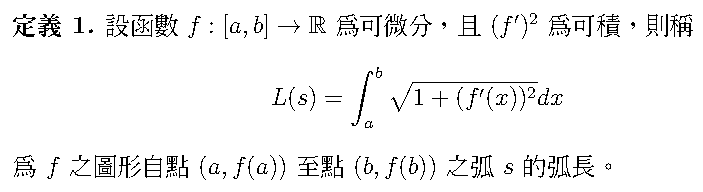
\includegraphics{cmath01}
\end{quote}

其中 {\ttfamily theoremstyle} 有三種 style,{\ttfamily plain, difinition, remark},預設使用的是 {\ttfamily plain},即定理名稱會用粗體字,內文則是 italic 斜體字,但這在中文並不適當,所以改由 {\ttfamily remark} style 來排版。要注意的是定理環境內的 {\ttfamily plain} style 雖然使用 italic 字型,但他並沒有進入數學模式,因此裡頭的數學式子仍然要進入數學模式來排版。另外,實數的那個特殊符號 $\mathbb{R}$ 要引用 {\sffamily amssymb} package 才會有,這也是美國數學協會\index{美國數學協會}發展的。


{\sffamily amsthm} 另提供了 \verb|\theoremstyle|\index{theoremstyle@\verb=\theoremstyle=} 給使用自行定義除了 {\ttfamily plain}、{\ttfamily definition} 及 {\ttfamily remark} 三種形式外的 style。另外,\LaTeX{} 本身的工具組也提供了一個 {\sffamily theorem} 巨集套件,能更有彈性的來細部微調,也有現成的指令,可以去改變所要使用的字體,可以參考系統上就有的 {\ttfamily theorem.dvi} 這個說明檔。

\section{數學模式中的字型及空間調整}

我們前面已有談到調整數學模式字體大小的四個指令。這裡我們再來看看其他的調整指令。

\subsection{數學字體的改變}

以下的指令,相信大家從他的簡寫就可以知道意思:

\begin{quote}
  \begin{tabular}{lll}
    指令                    & 作用        & 實例              \\
    \hline
    \verb|\mathrm| & 正常字體    & $\mathrm{ABCabc}$ \\
    \verb|\mathtt| & 打字機字族  & $\mathtt{ABCabc}$ \\
    \verb|\mathbf| & 粗體字      & $\mathbf{ABCabc}$ \\
    \verb|\mathsf| & sans serif  & $\mathsf{ABCabc}$ \\
    \verb|\mathit| & italic 斜體 & $\mathit{ABCabc}$ \\
    \verb|\mathcal| & 數學花體字  & $\mathcal{ABC}$
  \end{tabular}
\end{quote}

其他的套件會有更多的不同字體,請參考系統裡頭的 {\ttfamily symbols-a4.pdf}。要注意的是,有些字型並不是都完全有各種字體組合,像花體字並沒有小寫字母。

\subsection{數學模式中調整間距}

正常情況下,數學模式中的空間調整應不必使用者去操心,但程式畢竟不會思考,有些特殊場合仍然需要人為的調整。

\begin{quote}
  \begin{tabular}{llll}
    指令                    & 作用                   & 指令                    & 作用                 \\
    \hline
    \verb|\quad| & 空出一個 em 單位的空白 & \verb|\qquad| & 空出兩個 em 的空白   \\
    \verb|\,| & 加入 1/6 quad 的空白   & \verb|\!| & 減去 1/6 quad 的空白 \\
    \verb|\;| & 加入 5/18 quad 的空白  & \verb|\:| & 加入 2/9 quad 的空白
  \end{tabular}
\end{quote}

其中 \verb|\,|、\verb|\quad| 及 \verb|\qquad| 可以用在一般的文字模式及數學模式,其他的只能使用在數學模式中。我們把上一個弧長定義的例子來試著調整一下:

\begin{quote}
  \begin{verbatim}
 ...
\begin{cdefi}
設函數 $f:[a,b]\rightarrow{\mathbb R}$ 為可微分,且 $(f')^2$ 為可積,則稱
\[
L(s)=\int^b_a\!\sqrt{1+(f'(x))^2}\,dx
\]
為 $f$ 之圖形自點 $(a,f(a))$ 至點 $(b,f(b))$ 之弧 $s$ 的弧長。
\end{cdefi}
 ...
\end{verbatim}
\end{quote}

排版出來的結果是:

\begin{quote}
  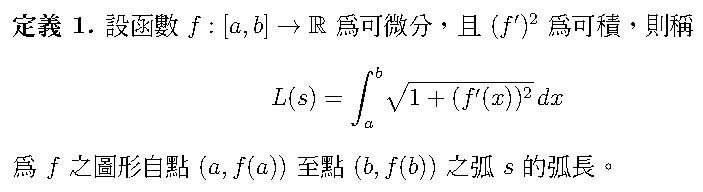
\includegraphics{cmath02}
\end{quote}

但是,要注意的是,如果文章有點長,數學式子也不少,那一定要注意整體的一致性,要調整的話就全文相同的地方都要去調整,否則就使用預設值就可以了,至少他不會太離譜。